\documentclass[tikz]{standalone}

% tikz
\usepackage{tikz, pgfplots}
% i wish external worked but idk it sucks
%\usetikzlibrary{external}
%\tikzexternalize[prefix=figures/]

% for function graph
\usetikzlibrary{positioning}
\usetikzlibrary{shapes.geometric}
\usetikzlibrary{positioning}
\usetikzlibrary{shapes.misc}
\tikzset{
dot/.style = {circle, fill=#1, minimum size=5pt,
              inner sep=0pt, outer sep=0pt},
dot/.default = black % size of the circle diameter
}
\tikzset{cross/.style={cross out, draw=black, minimum size=2*(#1-\pgflinewidth), inner sep=0pt, outer sep=0pt},
%default radius will be 1pt. 
cross/.default={1pt}}

 % for braces
\usetikzlibrary{decorations.pathreplacing}
% for hashing area
\usetikzlibrary{patterns}
% tableaux var, signe
% source https://www.sqlpac.com/fr/documents/latex-package-tkz-tab-tikz-tableaux-de-signes-et-de-variations-de-fonctions.html
\usepackage{tkz-tab}
%%%%%%%%%%%%%%%%%%%%%%%%%%%%%%
% SELF MADE COLORS
%%%%%%%%%%%%%%%%%%%%%%%%%%%%%%


\definecolor{myg}{RGB}{56, 140, 70}
\definecolor{myb}{RGB}{45, 111, 177}
\definecolor{myr}{RGB}{199, 68, 64}
\definecolor{mytheorembg}{HTML}{F2F2F9}
\definecolor{mytheoremfr}{HTML}{00007B}
\definecolor{mylenmabg}{HTML}{FFFAF8}
\definecolor{mylenmafr}{HTML}{983b0f}
\definecolor{mypropbg}{HTML}{f2fbfc}
\definecolor{mypropfr}{HTML}{191971}
\definecolor{myexamplebg}{HTML}{F2FBF8}
\definecolor{myexamplefr}{HTML}{88D6D1}
\definecolor{myexampleti}{HTML}{2A7F7F}
\definecolor{mydefinitbg}{HTML}{E5E5FF}
\definecolor{mydefinitfr}{HTML}{3F3FA3}
\definecolor{notesgreen}{RGB}{0,162,0}
\definecolor{myp}{RGB}{197, 92, 212}
\definecolor{mygr}{HTML}{2C3338}
\definecolor{myred}{RGB}{127,0,0}
\definecolor{myyellow}{RGB}{169,121,69}
\definecolor{myexercisebg}{HTML}{F2FBF8}
\definecolor{myexercisefg}{HTML}{88D6D1}
\definecolor{doc}{RGB}{0,60,110}

% manim colors because they're beautiful
% https://docs.manim.community/en/stable/reference/manim.utils.color.manim_colors.html

\definecolor{BLACK}{HTML}{000000}\definecolor{BLUE}{HTML}{58C4DD}\definecolor{BLUE_A}{HTML}{C7E9F1}\definecolor{BLUE_B}{HTML}{9CDCEB}\definecolor{BLUE_C}{HTML}{58C4DD}\definecolor{BLUE_D}{HTML}{29ABCA}\definecolor{BLUE_E}{HTML}{236B8E}\definecolor{DARKER_GRAY}{HTML}{222222}\definecolor{DARKER_GREY}{HTML}{222222}\definecolor{DARK_BLUE}{HTML}{236B8E}\definecolor{DARK_BROWN}{HTML}{8B4513}\definecolor{DARK_GRAY}{HTML}{444444}\definecolor{DARK_GREY}{HTML}{444444}\definecolor{GOLD}{HTML}{F0AC5F}\definecolor{GOLD_A}{HTML}{F7C797}\definecolor{GOLD_B}{HTML}{F9B775}\definecolor{GOLD_C}{HTML}{F0AC5F}\definecolor{GOLD_D}{HTML}{E1A158}\definecolor{GOLD_E}{HTML}{C78D46}\definecolor{GRAY}{HTML}{888888}\definecolor{GRAY_A}{HTML}{DDDDDD}\definecolor{GRAY_B}{HTML}{BBBBBB}\definecolor{GRAY_BROWN}{HTML}{736357}\definecolor{GRAY_C}{HTML}{888888}\definecolor{GRAY_D}{HTML}{444444}\definecolor{GRAY_E}{HTML}{222222}\definecolor{GREEN}{HTML}{83C167}\definecolor{GREEN_A}{HTML}{C9E2AE}\definecolor{GREEN_B}{HTML}{A6CF8C}\definecolor{GREEN_C}{HTML}{83C167}\definecolor{GREEN_D}{HTML}{77B05D}\definecolor{GREEN_E}{HTML}{699C52}\definecolor{GREY}{HTML}{888888}\definecolor{GREY_A}{HTML}{DDDDDD}\definecolor{GREY_B}{HTML}{BBBBBB}\definecolor{GREY_BROWN}{HTML}{736357}\definecolor{GREY_C}{HTML}{888888}\definecolor{GREY_D}{HTML}{444444}\definecolor{GREY_E}{HTML}{222222}\definecolor{LIGHTER_GRAY}{HTML}{DDDDDD}\definecolor{LIGHTER_GREY}{HTML}{DDDDDD}\definecolor{LIGHT_BROWN}{HTML}{CD853F}\definecolor{LIGHT_GRAY}{HTML}{BBBBBB}\definecolor{LIGHT_GREY}{HTML}{BBBBBB}\definecolor{LIGHT_PINK}{HTML}{DC75CD}\definecolor{LOGO_BLACK}{HTML}{343434}\definecolor{LOGO_BLUE}{HTML}{525893}\definecolor{LOGO_GREEN}{HTML}{87C2A5}\definecolor{LOGO_RED}{HTML}{E07A5F}\definecolor{LOGO_WHITE}{HTML}{ECE7E2}\definecolor{MAROON}{HTML}{C55F73}\definecolor{MAROON_A}{HTML}{ECABC1}\definecolor{MAROON_B}{HTML}{EC92AB}\definecolor{MAROON_C}{HTML}{C55F73}\definecolor{MAROON_D}{HTML}{A24D61}\definecolor{MAROON_E}{HTML}{94424F}\definecolor{ORANGE}{HTML}{FF862F}\definecolor{PINK}{HTML}{D147BD}\definecolor{PURE_BLUE}{HTML}{0000FF}\definecolor{PURE_GREEN}{HTML}{00FF00}\definecolor{PURE_RED}{HTML}{FF0000}\definecolor{PURPLE}{HTML}{9A72AC}\definecolor{PURPLE_A}{HTML}{CAA3E8}\definecolor{PURPLE_B}{HTML}{B189C6}\definecolor{PURPLE_C}{HTML}{9A72AC}\definecolor{PURPLE_D}{HTML}{715582}\definecolor{PURPLE_E}{HTML}{644172}\definecolor{RED}{HTML}{FC6255}\definecolor{RED_A}{HTML}{F7A1A3}\definecolor{RED_B}{HTML}{FF8080}\definecolor{RED_C}{HTML}{FC6255}\definecolor{RED_D}{HTML}{E65A4C}\definecolor{RED_E}{HTML}{CF5044}\definecolor{TEAL}{HTML}{5CD0B3}\definecolor{TEAL_A}{HTML}{ACEAD7}\definecolor{TEAL_B}{HTML}{76DDC0}\definecolor{TEAL_C}{HTML}{5CD0B3}\definecolor{TEAL_D}{HTML}{55C1A7}\definecolor{TEAL_E}{HTML}{49A88F}\definecolor{WHITE}{HTML}{FFFFFF}\definecolor{YELLOW}{HTML}{FFFF00}\definecolor{YELLOW_A}{HTML}{FFF1B6}\definecolor{YELLOW_B}{HTML}{FFEA94}\definecolor{YELLOW_C}{HTML}{FFFF00}\definecolor{YELLOW_D}{HTML}{F4D345}\definecolor{YELLOW_E}{HTML}{E8C11C}

% Schwartz
\renewcommand{\S}{\mathcal{S}} % \S est le signe paragraphe normalement

% corps
\newcommand{\C}{\mathcal{C}}
\newcommand{\R}{\mathbb{R}}
\newcommand{\Rnn}{\mathbb{R}^{2n}}
\newcommand{\Z}{\mathbb{Z}}
\newcommand{\N}{\mathbb{N}}
\newcommand{\Q}{\mathbb{Q}}

% domain
\newcommand{\D}{\mathcal{D}}

% order notations
\renewcommand{\O}{\mathcal{O}}

% japanese bracket
\newcommand{\japb}[1]{\langle #1 \rangle}

% arrows over partial derivatives
\newcommand{\lp}{\overleftarrow{\partial}}
\newcommand{\rp}{\overrightarrow{\partial}}

% quantization
\newcommand{\h}{\hbar}
\newcommand{\Opht}{\textrm{Op}_{\h}^{t}}
\newcommand{\Op}[2][\hbar]{\textrm{Op}_{#1}^{#2}}

% omega functions
\newcommand{\omegap}[2][\rho_0]{\omega(\partial_{#1},\partial_{#2})}
\newcommand{\omegar}[2][\rho_0]{\omega(#1,#2)}

\begin{document}
%
	% page 1
	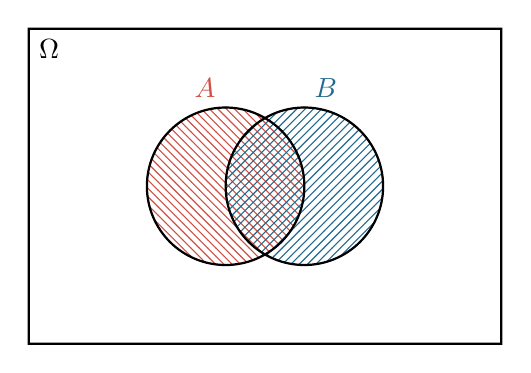
\begin{tikzpicture}[fill=gray, scale=1]
		% left hand
		\scope
		\draw[pattern=north west lines, pattern color=RED_E] (-.5,0) circle (1);
		\endscope
		% right hand
		\scope
		\draw[pattern=north east lines, pattern color=BLUE_E] (.5,0) circle (1);
		\endscope
		% outline
		\draw[thick] (-.5,0) circle (1) (-.5,1)  node [text=black,above left, RED_E] {$A$}
		      (.5,0) circle (1) (.5,1)  node [text=black,above right, BLUE_E] {$B$}
		      (3,-2) rectangle (-3,2) node [text=black,below right] {$\Omega$};
		%\draw (.5,0) node [text=black] {$A \cap B$};
	\end{tikzpicture}
	% page 2
	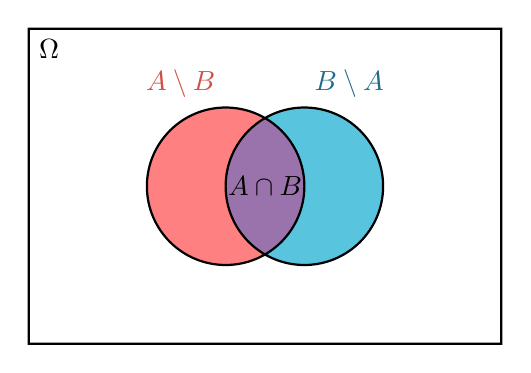
\begin{tikzpicture}[fill=gray, scale=1]
		% intersection
		\scope
		\fill[PURPLE] (-.5,0) circle (1);
		\endscope
		% left hand
		\scope
		\clip (-3,-2) rectangle (3,2)
		      (.5,0) circle (1);
		\fill[RED_B] (-.5,0) circle (1);
		\endscope
		% right hand
		\scope
		\clip (-3,-2) rectangle (3,2)
		      (-.5,0) circle (1);
		\fill[BLUE_C] (.5,0) circle (1);
		\endscope
		% outline
		\draw[thick] (-.5,0) circle (1) (-.5,1)  node [above left, RED_E] {$A\setminus B$}
		      (.5,0) circle (1) (.5,1)  node [above right, BLUE_E] {$B\setminus A$}
		      (3,-2) rectangle (-3,2) node [below right] {$\Omega$};
		\draw (0,0) node [black] {$A \cap B$};
	\end{tikzpicture}
	% page 3
	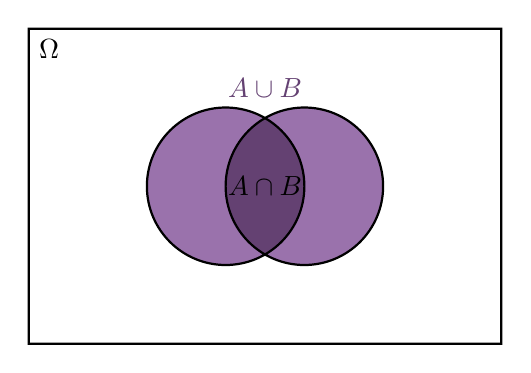
\begin{tikzpicture}[fill=gray, scale=1]
		% intersection
		\scope
		\fill[PURPLE_E] (-.5,0) circle (1);
		\endscope
		% left hand
		\scope
		\clip (-3,-2) rectangle (3,2)
		      (.5,0) circle (1);
		\fill[PURPLE] (-.5,0) circle (1);
		\endscope
		% right hand
		\scope
		\clip (-3,-2) rectangle (3,2)
		      (-.5,0) circle (1);
		\fill[PURPLE] (.5,0) circle (1);
		\endscope
		% outline
		\draw[thick] (-.5,0) circle (1) (-.5,1) 
		      (.5,0) circle (1) (.5,1) 
		      (3,-2) rectangle (-3,2) node [text=black,below right] {$\Omega$};
		\draw (0,1) node [text=black, above, PURPLE_E] {$A \cup B$};
		\draw (0,0) node [text=black] {$A \cap B$};
	\end{tikzpicture}
	
	% page 4
	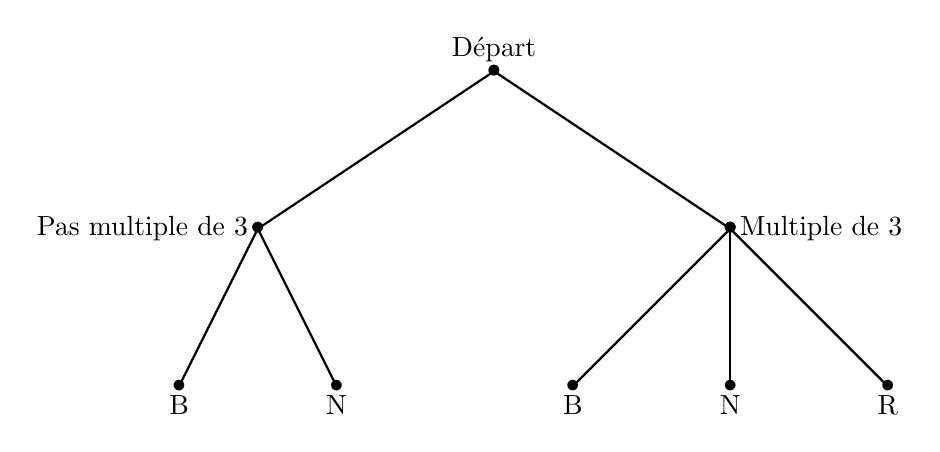
\begin{tikzpicture}
		% depth 1
		\foreach \i in {-3, 3}
		\draw[-, thick, black] (0,0) node {$\bullet$} -- (\i,-2);
		% depth 2
		\foreach \i in {3} \foreach \j in {-2, 0, 2}
			\draw[-, thick, black] (\i,-2) node {$\bullet$} -- (\i+\j,-4) node {$\bullet$};
			
		\foreach \i in {-3} \foreach \j in {-1, 1}
			\draw[-, thick, black] (\i,-2) node {$\bullet$} -- (\i+\j,-4) node {$\bullet$};
			
		\draw (0,0) node[above] {Départ};
		\draw (3,-2) node[right] {Multiple de $3$};
		\draw (-3,-2) node[left] {Pas multiple de $3$};
		\draw (-4,-4) node[below] {B};
		\draw (-2,-4) node[below] {N};
		\draw (1,-4) node[below] {B};
		\draw (3,-4) node[below] {N};
		\draw (5,-4) node[below] {R};
	\end{tikzpicture}
	
	% page 5
	\begin{tikzpicture}
		% depth 1
		\foreach \i in {-3, 3}
		\draw[-, thick, black] (0,0) node {$\bullet$} -- (\i,-2);
		% depth 2
		\foreach \i in {3} \foreach \j in {-2, 0, 2}
			\draw[-, thick, black] (\i,-2) node {$\bullet$} -- (\i+\j,-4) node {$\bullet$};
			
		\foreach \i in {-3} \foreach \j in {-1, 1}
			\draw[-, thick, black] (\i,-2) node {$\bullet$} -- (\i+\j,-4) node {$\bullet$};
			
		\draw (0,0) node[above] {Départ};
		\draw (3,-2) node[right] {Multiple de $3$};
		\draw (-3,-2) node[left] {Pas multiple de $3$};
		\draw (-4,-4) node[below] {B};
		\draw (-2,-4) node[below] {N};
		\draw (1,-4) node[below] {B};
		\draw (3,-4) node[below] {N};
		\draw (5,-4) node[below] {R};
		
		\draw (-1.5, -1) node[above left] {$\dfrac23$};
		\draw (1.5, -1) node[above right] {$\dfrac13$};
		
		\draw (-3.5, -3.25) node[above left] {$\frac25$};
		\draw (-2.5, -3.25) node[above right] {$\frac35$};
		
		\draw (2, -3.25) node[above left] {$\frac25$};
		\draw (3, -3.25) node[right] {$\frac3{10}$};
		\draw (4, -3.25) node[above right] {$\frac3{10}$};
	\end{tikzpicture}
	% page 6
	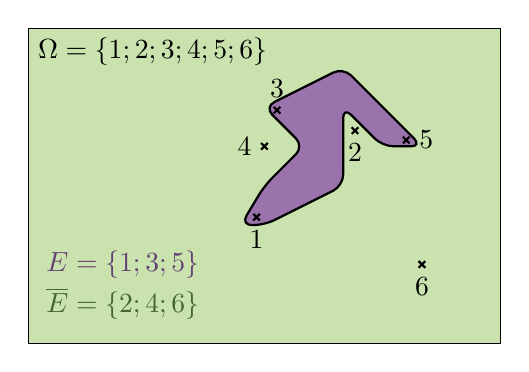
\begin{tikzpicture}[fill=gray, scale=1]
		% univers
		\draw[fill=GREEN_A] (3,-2) rectangle (-3,2) node [below right] {$\Omega = \{ 1 ; 2 ; 3 ; 4 ; 5 ; 6 \}$};
		
		% E
		\draw[rounded corners, fill = PURPLE, thick] (0,0) -- (.5,.5) -- (0,1) -- (1,1.5) -- (1.5,1) -- (2, .5) -- (1.5,.5) -- (1,1) -- (1,0) -- (0,-.5) -- (-.3,-.5) -- cycle;
		\draw[PURPLE_E] (-1.8,-1) node {$E = \{1 ; 3 ; 5\}$};
		\draw[GREEN_E!65!BLACK] (-1.8,-1.5) node {$\overline{E} = \{2 ; 4 ; 6\}$};
		% wish that GREEN_E would work but it's hard to read
		
		% e in E
		\node[cross=2pt, label=below:1, thick] at (-.1,-.4){};
		\node[cross=2pt, label=above:3, thick] at (.16,.96){};
		\node[cross=2pt, label=right:5, thick] at (1.8,.58){};
		
		% e notin E
		\node[cross=2pt, label=below:2, thick] at (1.15,.7){};
		\node[cross=2pt, label=left:4, thick] at (0,.5){};
		\node[cross=2pt, label=below:6, thick] at (2,-1){};
	\end{tikzpicture}
	% page 7
	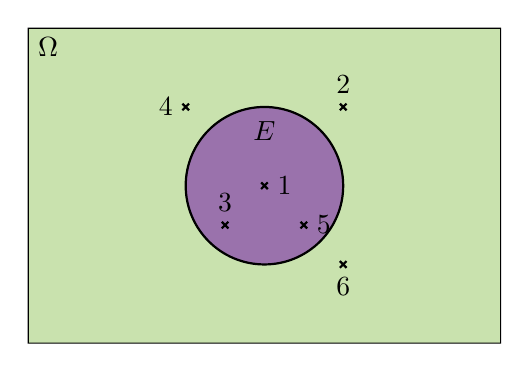
\begin{tikzpicture}[fill=gray, scale=1]
		% outline
		\draw[fill=GREEN_A] (0,0) circle (1)
		      (3,-2) rectangle (-3,2) node [text=black,below right] {$\Omega$};
		% E
		\scope
		\fill[PURPLE] (0,0) circle (1);
		\endscope
		\draw[thick] (0,0) circle (1);
		      
		% e in E
		\draw (0,.7) node [text=black] {$E$};
		\node[cross=2pt, label=right:1, thick] at (0,0){};
		\node[cross=2pt, label=above:3, thick] at (-.5,-.5){};
		\node[cross=2pt, label=right:5, thick] at (.5,-.5){};
		% e notin E
		%\draw (2,0) node [text=black] {$\overline{E}$};
		\node[cross=2pt, label=above:2, thick] at (1,1){};
		\node[cross=2pt, label=left:4, thick] at (-1,1){};
		\node[cross=2pt, label=below:6, thick] at (1,-1){};
	\end{tikzpicture}
%
\end{document}